\documentclass[aspectratio=169]{beamer}
\setbeamertemplate{navigation symbols}{} % don't use navigation tools on slides
% \usetheme{LMT}

\usepackage[utf8]{inputenc}
\usepackage{pdfpc-commands}
\usepackage{multimedia}
\usepackage{listings}
\usepackage{default}

\setbeamersize{text margin left=0.6cm,text margin right=0.6cm}
\setbeamercolor{frametitle}{fg=black}
\setbeamercolor{section in toc}{fg=black}
\setbeamertemplate{frametitle}{\color{black}\bfseries\insertframetitle\par\vskip-6pt{\color{gray}\hrulefill}}

\lstset{language=C++,
  basicstyle=\ttfamily,
  keywordstyle=\color{blue}\ttfamily,
  stringstyle=\color{red}\ttfamily,
  commentstyle=\color{green}\ttfamily,
  morecomment=[l][\color{magenta}]{\#}
}

\AtBeginSection[]{
  \begin{frame}{Sommaire}
    \tableofcontents[currentsection]
  \end{frame} 
}

\begin{document}

\begin{frame}
    \begin{center}
        {\huge High Performance Computing of Power Diagrams}

        \bigskip
        {\large Applications to Semi-Discrete Optimal Transport}
      
        \vfill
        {(MAGA days, November 21, 2019, Hugo Leclerc)}
    \end{center}
\end{frame}

% ---------------------------------------------------------------------------------------
\section{}

\begin{frame}
    \frametitle{The world needs power diagrams !}

    \begin{minipage}{0.5\textwidth}
        Problem to solve: what is the optimal way to transport a density to a set of diracs with equal mass ? 
        
        \bigskip
        Quadratic cost (euclidian distance) $\Rightarrow$ \textit{attributions} are defined by power diagrams !
        
        \hfill
    \end{minipage}
    \kern 0.5cm
    \begin{minipage}{0.45\textwidth}
        \begin{center}
            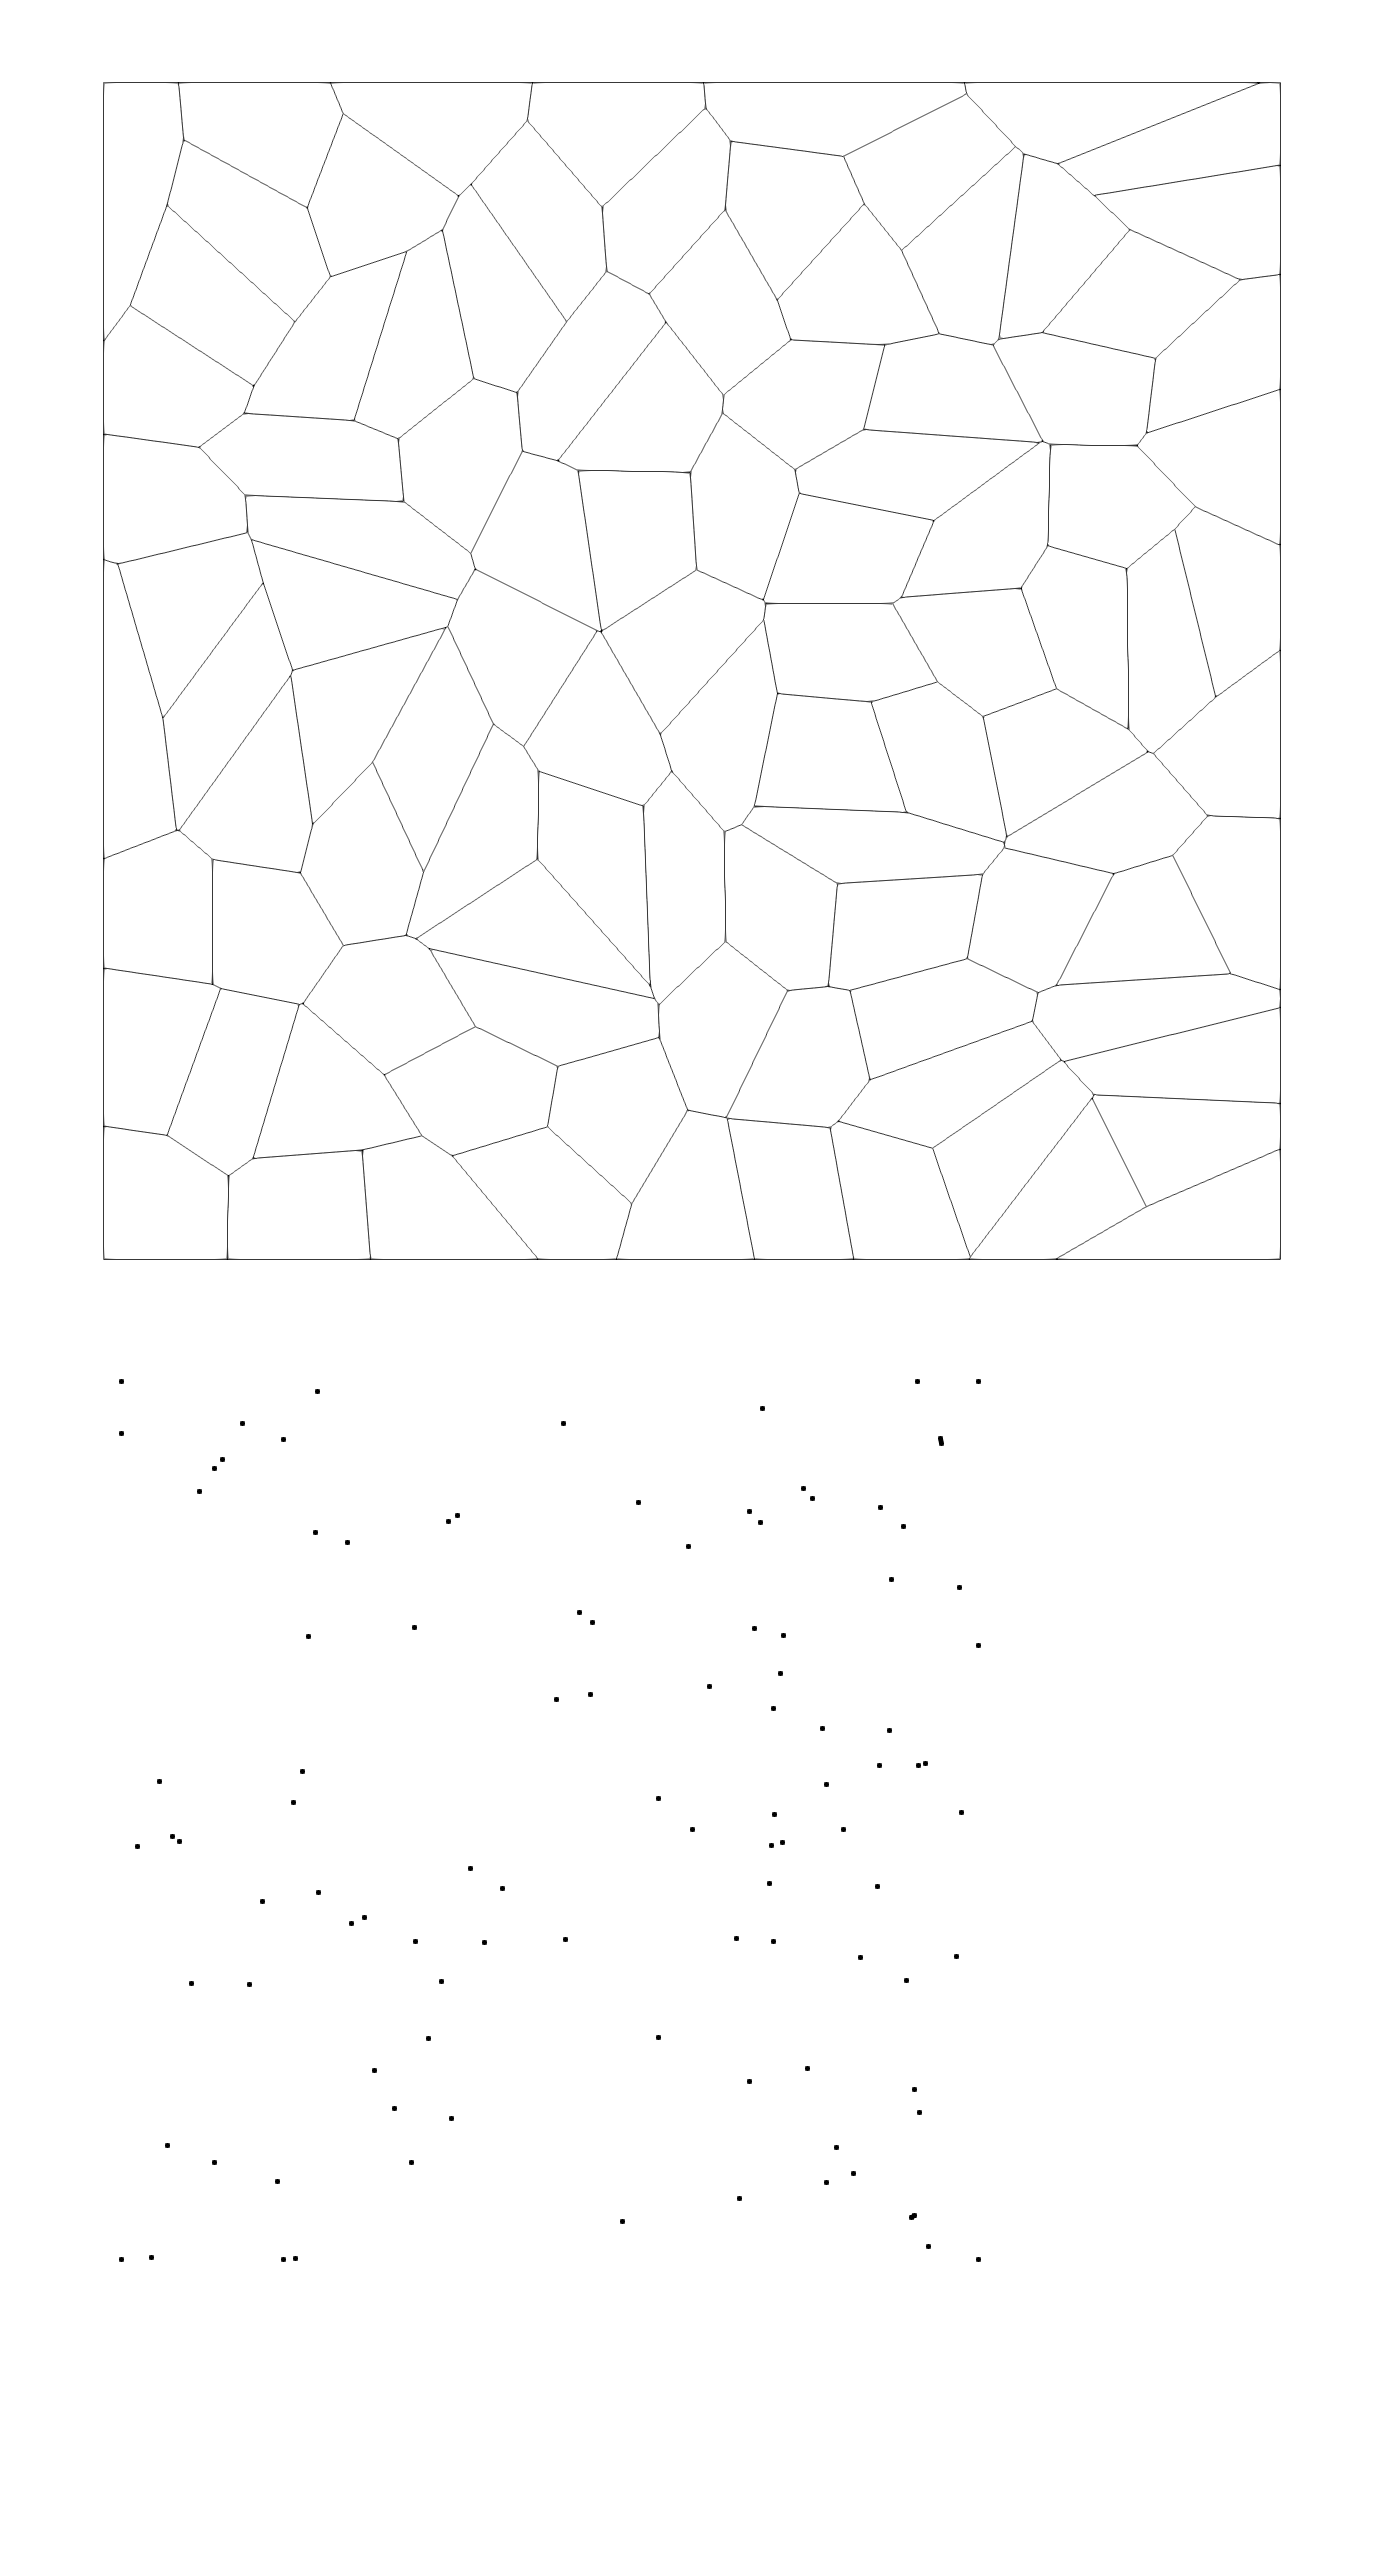
\includegraphics[height=0.8\textheight]{img/pd.png}
        \end{center}
    \end{minipage}
\end{frame}

\begin{frame}
    \frametitle{The world needs efficient power diagram computations !}

    Lot of work done before. Extra-fast computation for the generic case...

    ... which cover cases (e.g. exact connectivity) that are not useful for SDOT (we need integrals).
    
    Most of the libraries are designed to give an exact connectivity...
        \\{\hfill extra cost on CPU}
        \\{\hfill ... using (mostly) sequential algorithms}
    
    \vfill
    But it's not mandatory for SDOT !
    
    
    \vfill
    $\Rightarrow$ Prop
\end{frame}



\begin{frame}
    \frametitle{Principle}

\end{frame}


\begin{frame}
    \frametitle{}

\end{frame}


 
% ---------------------------------------------------------------------------------------
\section{Conclusions et perspectives}

\begin{frame}
    \frametitle{Conclusions}

    Il est possible de rapprocher \textit{encore} la programmation des maths appliquées
    \begin{itemize}
        \item pour perdre moins de temps
        \item pour mieux séparer les difficultés
        \item et moins se déformer l'esprit
    \end{itemize}
    
    \vfill
    Illustration avec l'évaluation paresseuse~: 
    \begin{itemize}
        \item simplification extrême des écritures 
        \item avec sémantique significativement plus précise
        \item adaptations automatiques et évolutives en fonction du hardware
        \item programmation symbolique
    \end{itemize}
\end{frame}


\begin{frame}
    \frametitle{Perspectives}

    \begin{itemize}
        \item Différentiations (positions initiales, bords, ...) et adaptations pour le transport optimal (semi-discret)
        \vfill
        \item Simplification des représentations pour les reconstructions tomographiques
        \vfill
        \item Plus grande palette de schémas d'intégration (collant aux équations)
        \vfill
        \item Extraction de propriétés mathématiques
    \end{itemize}
\end{frame}


\end{document}
